
\section{Application and System Analysis}
\label{sec:evaluation}

With a firm understanding of which of several ACID and distributed
consistency properties are available and which are not, we begin to
understand their implications for existing algorithms, applications,
and deployments. Specifically:

\begin{myenumerate}
\item We revisit traditional database concurrency control with a focus
  on coordination costs and on high availability.
\item We examine the properties required by a realistic OLTP
  application patterned on the TPC-C benchmark.
\item We perform a brief experimental evaluation of HAT versus non-HAT
  properties on public cloud infrastructure.
\end{myenumerate}

\subsection{Existing Algorithms}

Many existing database transaction and concurrency control algorithms
are not designed for high availability. These algorithms often presume
a single-server deployment or the requirement for serializability. As
a consequence, traditional transaction processing systems are not
well-optimized for a HAT context. In this section, we briefly discuss
design decisions and algorithmic details that preclude high
availability.

\vspace{.5em}\noindent\textbf{Serializablity} To establish a serial
order on transactions, all existing algorithms for achieving
serializability of general-purpose read-write transactions in a
distributed setting~\cite{bernstein-book} may require at least one
round trip time (RTT) before committing. As an example, traditional
two-phase locking for a transaction of length $T$ requires $T$
\texttt{lock} operations and at least one \texttt{unlock} operation.
Each of these operations requires coordination, either with other
database replicas or with a lock service. If the coordination
mechanism for locking is unavailable, transactions cannot
commit. Similarly, optimistic concurrency control requires contacting
a validation service, while deterministic transaction
scheduling~\cite{deterministic-scheduling} requires a
scheduler. Serializability under multi-version concurrency control
fares somewhat better but still requires checking for update
conflicts.

Perhaps unsurprisingly, the reliance on a globally agreed total order
necessitates a minimum of one round-trip to a designated master or
coordination service for each of these classic algorithms.  This is
intuitively a consequence of serializability's lack of high
availability~\cite{davidson-survey} (or, as we have shown, reliance on
preventing Lost Update and Write Skew).  The cost of the (minimum one)
round trip will be determined by the deployment environment, as we saw
in Section~\ref{sec:motivation}.

\vspace{.5em}\noindent\textbf{Non-serializablity} Perhaps
interestingly, many existing distributed implementations of weak
isolation are not highly available. Lock-based proposals such as those
used to provide weak isolation in Gray's original
proposal~\cite{gray-isolation} do not degrade gracefully in the
presence of partial failure. (Note, however, that lock-based protocols
\textit{do} offer the benefit of recency guarantees.) While
multi-versioned storage systems allow for a variety of transactional
guarantees, we have not seen proposals for truly weak isolation (e.g.,
non-``tentative update'' schemes) in this context. Chan and Gray's
read-only transactions provide read-only transactions with item-cut
isolation, causal consistency, and transactional atomicity but are
unavailable in the presence of coordinator failure~\cite{readonly},
similar to read-only and write-only transactions more recently
proposed by Eiger~\cite{eiger}.  Bolt-on causal
consistency~\cite{bolton}, Brantner's S3 database~\cite{kraska-s3},
and Bayou~\cite{sessionguarantees} can all provide variants of the
above model with high availability, but none provide this HAT
functionality without substantial modification; Swift~\cite{swift} is
closest to providing full HAT operation in a sticky
context. Similarly, the MDCC~\cite{mdcc} protocol offers Read
Committed isolation with Lost Update avoidance but is similarly
unavailable due to its reliance on preventing write conflicts.

As we have seen, it is possible to implement many guarantees weaker
than serializability---including guarantees that are achievable with
high availability---and not achieve high availability. We expect that
further understanding the trade-offs between semantic strength,
performance, and storage and metadata requirements will remain an area
of active research for the foreseeable future.

\subsection{Application Requirements}

Thus far, we have largely ignored the question of which applications
require semantics which are unavailable to HATs. As we showed in
Section~\ref{sec:hats}, the main cost of choosing HATs comes in the
inability to prevent Lost Update, Write Skew, and provide recency
bounds. In this section, we attempt to understand when these
guarantees matter both abstractly and by the use of a representative
customer order transaction application patterned off of the TPC-C
benchmark~\cite{tpcc}.

\vspace{.5em}\noindent\textbf{Commutativity and Monotonicity} Recent
work on the CALM Theorem~\cite{calm}, Lattice-based state
update~\cite{blooml}, and Commutative and Replicated Data
Types~\cite{crdt} demonstrates that, if updates logically commute,
then they can often be safely performed in different orders at
different locations in a distributed system. Accordingly, as long as
all writes are delivered to all replicas, then a system executing
monotonic logic with commutative operators may not suffer from
application-level consistency anomalies as a result of Lost Update or
Write Skew anomalies. However, applications with non-monotonic state
mutation will not, in general, be able to maintain application-level
consistency constraints. Similarly, applications requiring write
visibility between clients should opt for unavailability instead of
possibly missing a write visibility deadline.

\vspace{.5em}\noindent\textbf{TPC-C} Absent a necessary and sufficient
result describing exactly which application logics can be achieved
with high availability and to make these requirements more concrete,
we consider an example application: the TPC-C benchmark. Our goal is
\textit{not} to provide a performance analysis, as a HAT
configuration will be non-compliant. Rather, we examine the five
queries contained in the benchmarks---ostensibly representative of a
standard transaction processing application---to understand which are
achievable in a HAT context. Surprisingly, four of five can be
executed with HATs, while the fifth potentially requires unavailablity.

TPC-C consists of five transactions, capturing operation of a
real-world warehouse, including sales, payments, and deliveries. Two
transactions---\textit{Order-Status} and \textit{Stock-Level}---are
read-only and can be executed safely under HATs. Clients may read
stale data, but this does not violate TPC-C requirements and clients
will read their writes if they are sticky-available. Another
transaction type, \textit{Payment}, updates running balances for
warehouses, districts, and customer records as well as providing an
audit trail. The transaction is increment-only, so all balance
increase operations can commute, and TA allows the maintainence of any
foreign-key constraints (e.g., \texttt{UPDATE/DELETE CASCADE}).

While three out of five transactions have been easily achievable with
HATs, the remaining two transactions---\textit{New-Order} and
\textit{Delivery}---are not so simple. The New-Order transaction
places an order for a variable quantity of data items, updating
warehouse stock as needed. It selects a sales district, assigns the
order an ID number, adjusts the remaining warehouse stock, and writes
a placeholder entry for the pending order. The Delivery transaction
represents the fulfillment of a New-Order: it deletes the order from
the pending list, updates the customer's balance, updates the order's
carrier ID and delivery time, and updates the customer balance.

There are three challenges that only allow HATs to place non-compliant
New-Orders and to fail on Payments. First, New-Order requires a unique
ID number for each order. We can create a unique number by, say,
concatenating the client ID and a timestamp. However, the TPC-C
specification requires order numbers to be \textit{sequentially}
assigned, which requires Lost Update. Accordingly, HATs cannot provide
compliant TPC-C execution but can maintain uniqueness
constraints. Second, the New-Order transaction decrements inventory
counts: what if the count becomes negative? Fortunately, TPC-C
New-Order restocks each item's inventory count (increments by 91) if
it would become negative as the result of placing an order. This means
that, even in the presence of concurrent New-Orders, an item's stock
will never fall below zero. This is TPC-C compliant, but a HAT system
might end up with substantially more stock than in a single-site
implementation. Third, delivery events are non-monotonic---deleting a
pending New-Order transaction---and should be idempotent in order to
avoid billing a customer twice; this implies a need to prevent Lost
Update. We can avoid this issue by moving the non-monotonicity to the
real world---the carrier that picks up the package for an order can
ensure that she is the only carrier who has done so---but cannot
provide a correct execution with HATs alone.

Throughout execution, TPC-C also requires the maintainence of several
integrity constraints. For example, Consistency Condition 1 (3.3.2.1)
requires that each warehouse's sales count must reflect the sum of its
subordinate sales districts. This integrity constraint spans two
tables but, given the ability to update rows in both tables atomically
via transactional atomicity, can be easily maintained. Consistency
Conditions 4 through 12 (3.3.2.4-12) can similarly be satisfied by
applying updates atomically across tables. Consistency Conditions 2
and 3 (3.3.2.2-3) concern order ID assignment and are more
problematic, as we have discussed.

In summary, many---but not all---TPC-C transactions are well-served by
HATs. The two problematic transactions---New-Order and Payment---rely
on non-monotonic state update. The former transaction can be modified
to ensure ID uniqueness at the expense of sequential per-district ID
ordering, while the latter is an inherently non-monotonic action
requiring external compensation or stronger consistency protocols. We
expect that, especially for read-dominated workloads found in many
online services, HAT guarantees will suffice for many application
transactions. Finally, while TPC-C is not subject to multi-key
anomalies, we note that many TPC-E isolation tests, such as one that
requires simultaneously modifying a product description and its image,
are also passable using HATs.

\subsection{Experimental Costs}

\begin{figure}
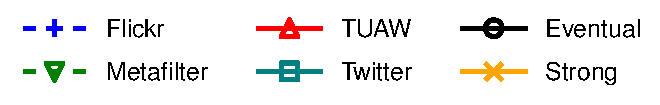
\includegraphics[width=.8\columnwidth]{figs/macrotracelegend.pdf}\vspace{-2mm}
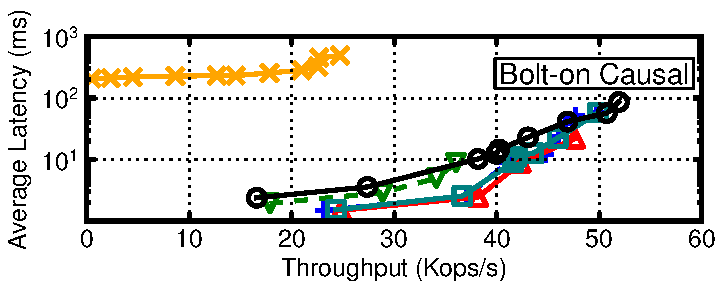
\includegraphics[width=\columnwidth]{figs/lat-thru-trace-K0-SCALEMACRO.pdf}
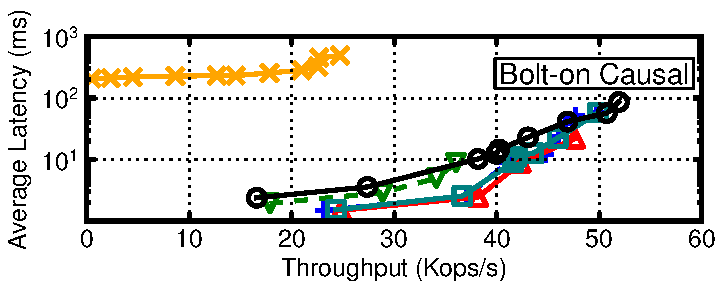
\includegraphics[width=\columnwidth]{figs/lat-thru-trace-K0-SCALEMACRO.pdf}
\caption{Latency-throughput for database operation on EC2 (DUMMY FIG)}
\label{fig:wan-exp}
\end{figure}

2.) We ran YCSB on EC2 (and maybe TPC-C if we have time) with a few models:
	- Eventual Consistency
	- Eventual consistency with a "master" for updates--simulates the lower bound on a non-HAT system.
	- Transactional Atomicity and Read Committed
	
	-This is going to look a lot like the ping tests: much higher latency for "non-HATs."
	-Our Naive 2PL implementation bottlenecks extremely quickly.
	-On, say, 5 servers, can get hundreds of thousands of TPS

	-Not meant as an exhaustive study, but validates our intuitions. Coordination costs of non-HAT systems are unaccounted for, will only go up, and we haven't even talked about availability.
